\input /users/davidmcallester/icloud/tex/SlidePreamble
\input /users/davidmcallester/icloud/tex/preamble

\begin{document}

{\Huge

  \centerline{\bf TTIC 31230, Fundamentals of Deep Learning}

  
\bigskip

\centerline{David McAllester, Autumn  2024}


\vfill

\centerline{\bf Theorem Proving}

\vfill
\vfill


\slide{MathZero?}

\centerline{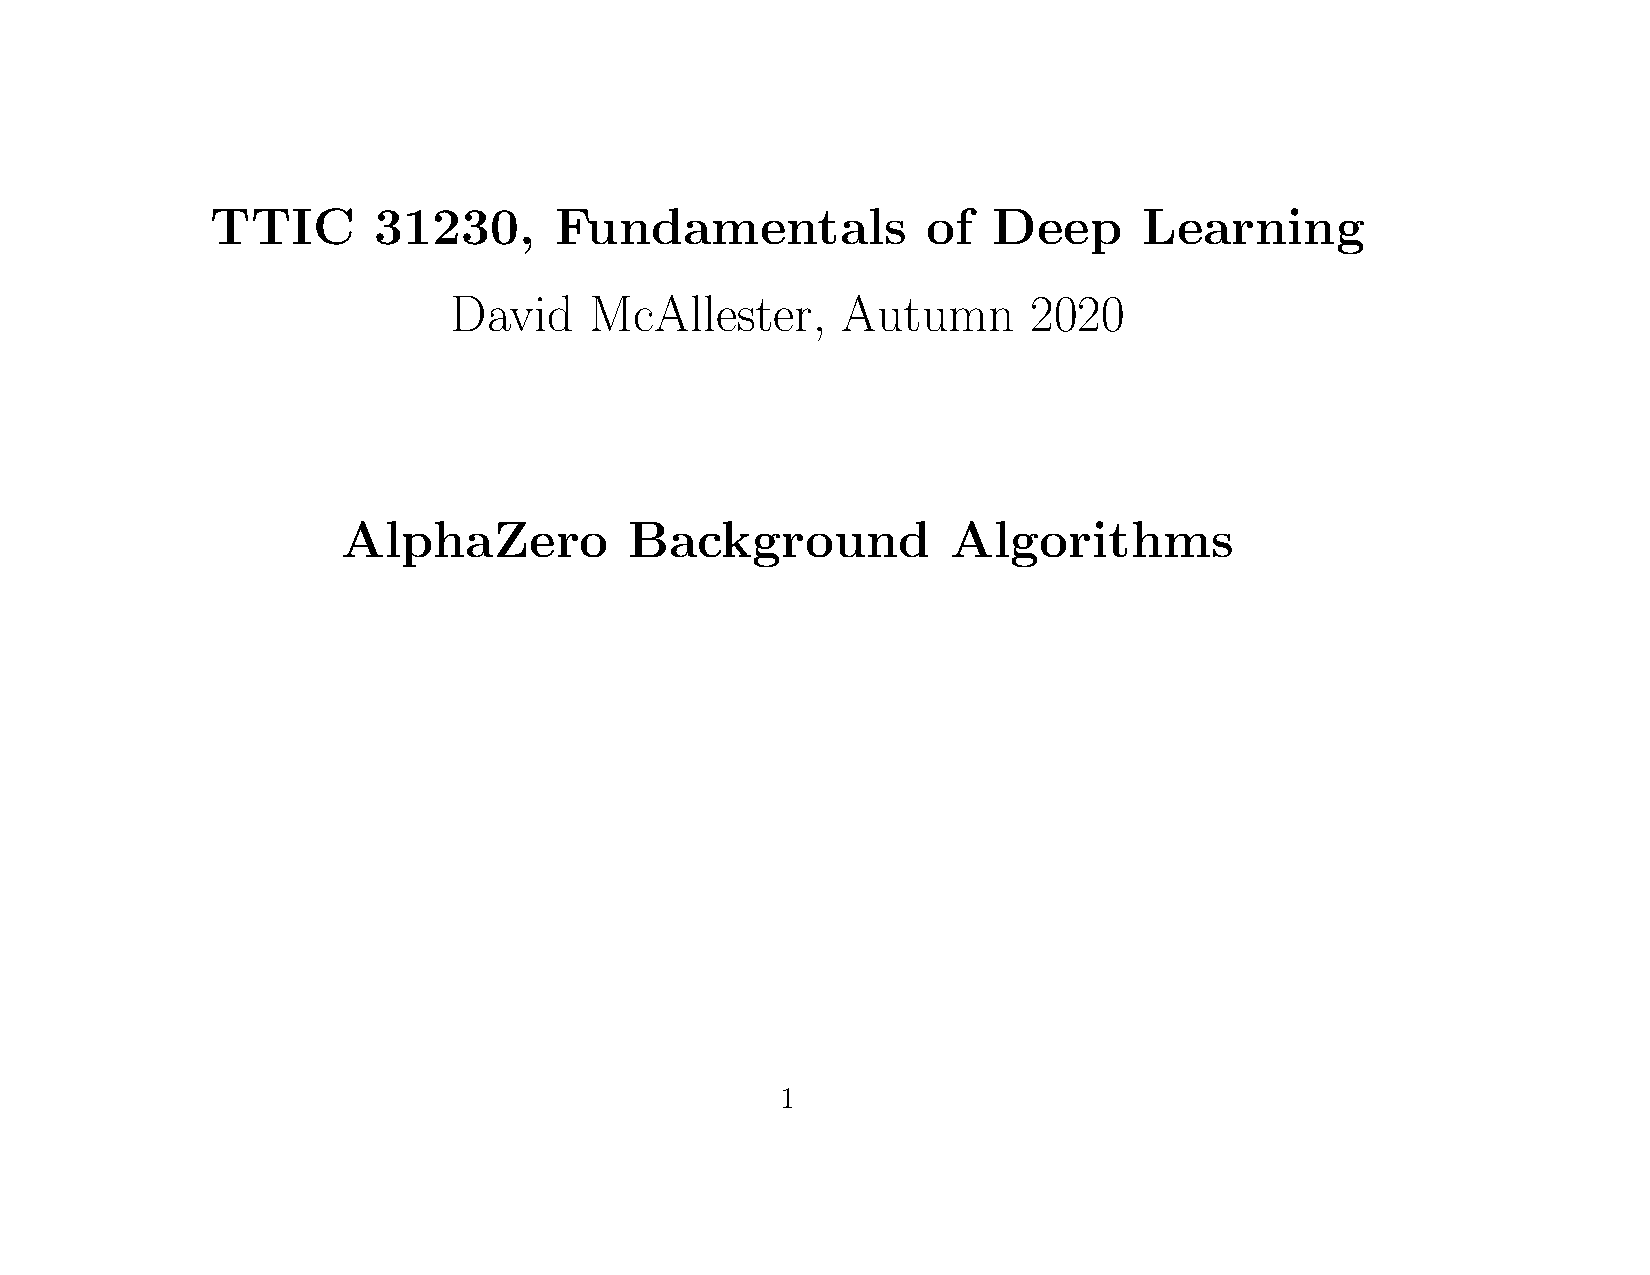
\includegraphics[height = 2.0in]{\images/alphago}}

\vfill

In 2017 AlphaZero learned to play Go, chess and shogi at a superhuman level given only the rules of the game.

\vfill
Lots of people have wondered whether something similar might be done for mathematics.

\slide{AlphaProof}

The IMO (International Math Olypiad) is an annual mathemamtics contest for high school students.

\vfill
Of the six problems in July 2024 IMO, DeepMind's AlphaGeometry solved the one geometry problem and AlphaProof solved three of the remaining five.

\vfill
The solutions were worth a silver medal.  However, AlphaProof took three days rather than the 1.5 hours humans get per problem.

\vfill
There is a blog post with a high level description (discussed below) but no paper has yet appeared.

\slide{Three Cultures}

{\bf Mathematicians (users)}: Building an AI system that can learn to play chess, Go or shogi is different from playing
chess, Go or shogi. Building a systems that can do mathematics different from doing mathematics.


\vfill
{\bf Deep Learning Researchers:} There is now a significant literature on using LLMs to generate formal proofs.

\vfill
{\bf Logicians:} The developers of formal verification systems that ensure correctness
are part of the formal methods community (programming languages, type theory, and formally sound automated reasoning).

\slide{Interest From Mathematicians}

Terence Tao (Fields Medalist) organized a group effort that machine verified one of his (coauthored) recent papers. (September 2023).

\vfill
Peter Scholze (Fields Medalist) organized a group effort that machine verified what he considered his most important theorem (2022).

\vfill
Tim Gowers (Fields Medalist) is now focusing on improving the level of automation in machine verfication systems.

\vfill
Kevin Buzzard has announced a project to machine verify Fermat's last theorem.

\slide{LLM Guided Provers}

\centerline{Generative Language Modeling for Automated Theorem Proving,}
\centerline{Polu and Sutskever, (Sept, 2020, OpenAI)}
%\centerline{(uses MetaMath rather than Lean)}

\vfill
AlphaProof, Deep Mind, July 2024, unpublished

\vfill
\centerline{DeepSeek-Prover-V1.5: Harnessing Proof Assistant Feedback}
\centerline{for Reinforcement Learning and Monte-Carlo Tree Search}
\centerline{Xin, et al., August 2024}

\slide{Logicians: The Lean System}

By far, the dominant system for ensuring correctness is Lean.

\vfill
{\bf Users:} Mathematician users, such as Terence Tao, Peter Scholze, and Kevin Buzzard, work directly in Lean with possible assistance
from LLMs used in the same way that programmers use LLMs -- to make suggestions.

\vfill
{\bf Deep Learning Researchers:} Deep learning researchers are almost exclusively using Lean to ensure correctness.

\vfill
{\bf Logicians:} I have built a system (Alfred) that is intended to be a compeitor for Lean.

\slide{Goals and Tactics}

I will call a statement that remains to be proved a goal.

\vfill
In Lean a tactic is a function that takes a set of goals and ``backward chains'' to produce a new set of goals.

\vfill
For a proof state $S$ and tactic $T$ we have that $T(S)$ is a new set of goals such that solving $T(S)$ solves $S$.

\slide{Goals and Tactics}

\vfill
For set of goals $S$ and tactic $T$ we have that $T(S)$ is a new set of goals such that solving $T(S)$ solves $S$.

\vfill
Example of tactics include:

\vfill
{\bf apply:} For applying a particular lemma under a certain instantiation

\vfill
{\bf simplify:} For simplifying an algebraic expression.

\vfill
{\bf induction:} For applying mathematical induction.

\vfill
{\bf show:} For showing a particular intermediate step that can then be added to the premises of a goal.

\slide{and-or Proof Trees}

Given a set of goals we can try to solve the goals seperately by applying a tactic to each individual goal.

\vfill
This results in an and-or search tree.  At an and node we need solve all the chidren and at an or node we need to
solve only one of the children.

\vfill
HyperTree Proof Search for Neural Theorem Proving, Lample et al., May 2022 (Meta).


\slide{and-or Proof Trees}

An and-or proof search is similar to chess or Go in that we can imagine two agents where one tries to prove the result and other tries to refute it.

\vfill
This is equivalent to min-max search where the maximizer proves and the minimizer refutes.

\vfill
We can then use $\alpha$-$\beta$ search, or Monte-Carlo tree search, or AlphaZero.

\slide{AlphaProof}

The blog post includes the following figure.

\centerline{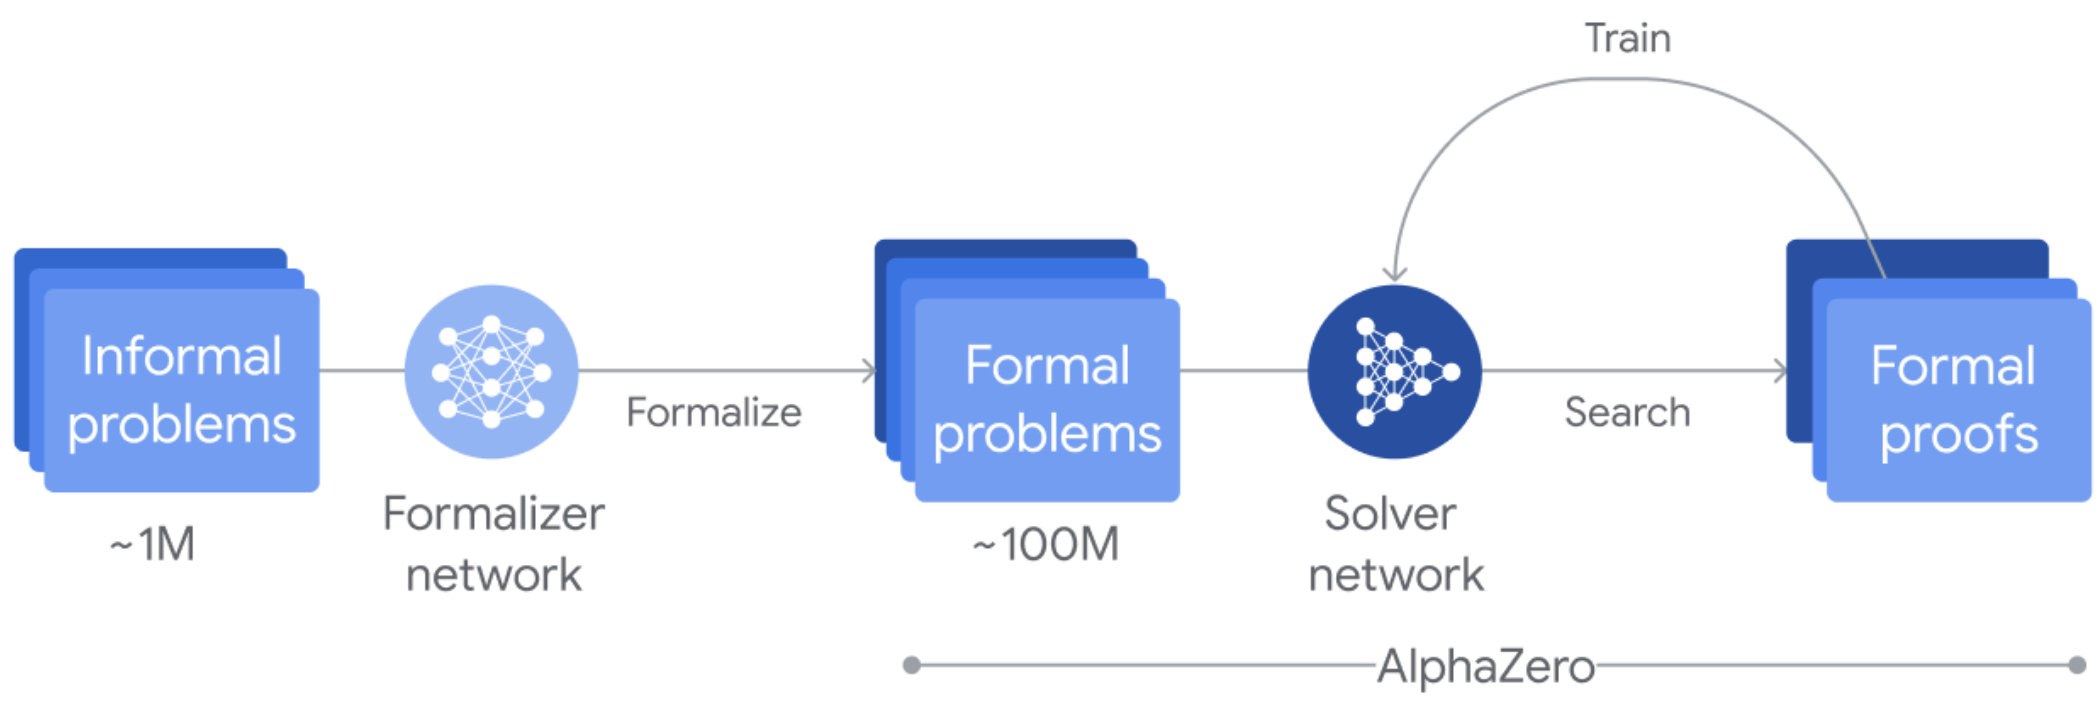
\includegraphics[width = 8in]{\images/AlphaProof}}

\vfill
For now we can only be sure about published systems.

\slide{Whole Proof Generation}

Baldur: Whole-Proof Generation and Repair with Large Language Models, First et al, March 2023, (UMass Amherst, Google, UIUC).

\vfill
One can repeatedly ask the language model to generate
a compete proof --- a sequence of tactics that solves the given goal.

\vfill
Whole proof generation is used as a subroutine in DeepSeek Prover.

\vfill
Whole proof generation is typically associated with or-branching tree search where each node is a set of subgoals.

\slide{DeepSeek1.5}

DeepSeek 1.5 appears to be the state of the art LLM-guided prover among those with a published paper.

\vfill
It uses whole proof generation but treats these as ``rollouts'' in an or-tree.  The steps in each generated whole proof
become new nodes in the or-tree and rollouts (whole proof generation) can be done from internal nodes.

\slide{DeepSeek 1.5}

\centerline{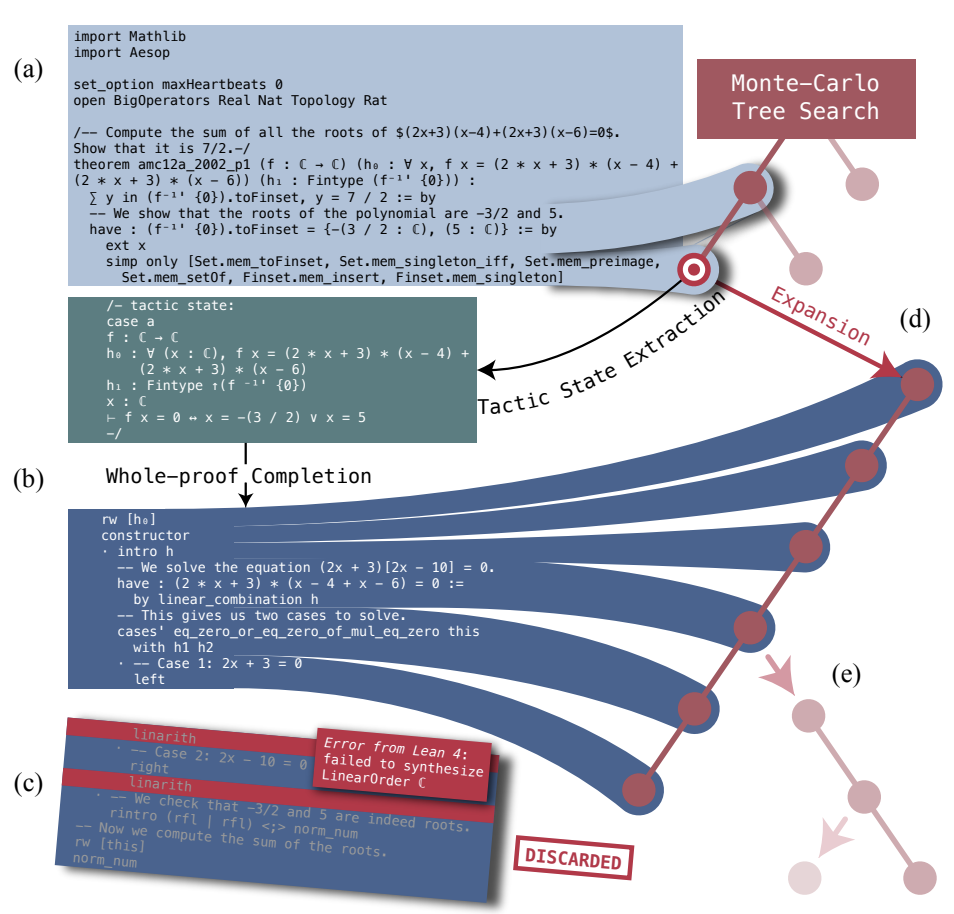
\includegraphics[height = 5in]{\images/DeepSeek1}}

\slide{English Comments and Intrinsic Reward}

DeepSeek uses monte-carlo tree search with an intrinsic reward for exploration (generating new nodes).


\vfill
DeepSeek inserts natural language comments for each tactic application which might help guide the proof.

\slide{Pretraining Corpus}

\centerline{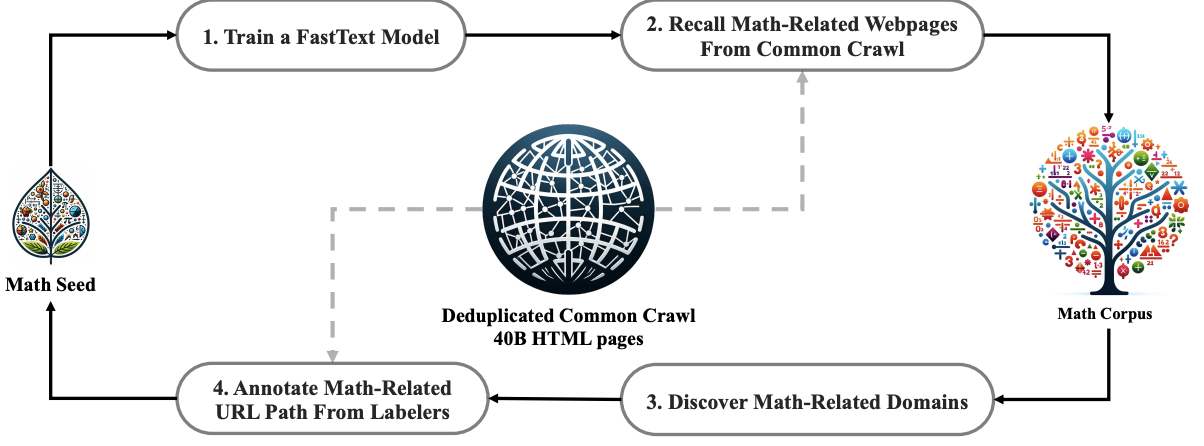
\includegraphics[width = 8in]{\images/DeepSeek3}}

\vfill
They collect 40B tokens of mathematical text.


\slide{Self Play Imitation Learning}

As they prove new formal theorems the new theorems are added to a database of proofs
used in ``imitation fine tuning''.

\vfill
\centerline{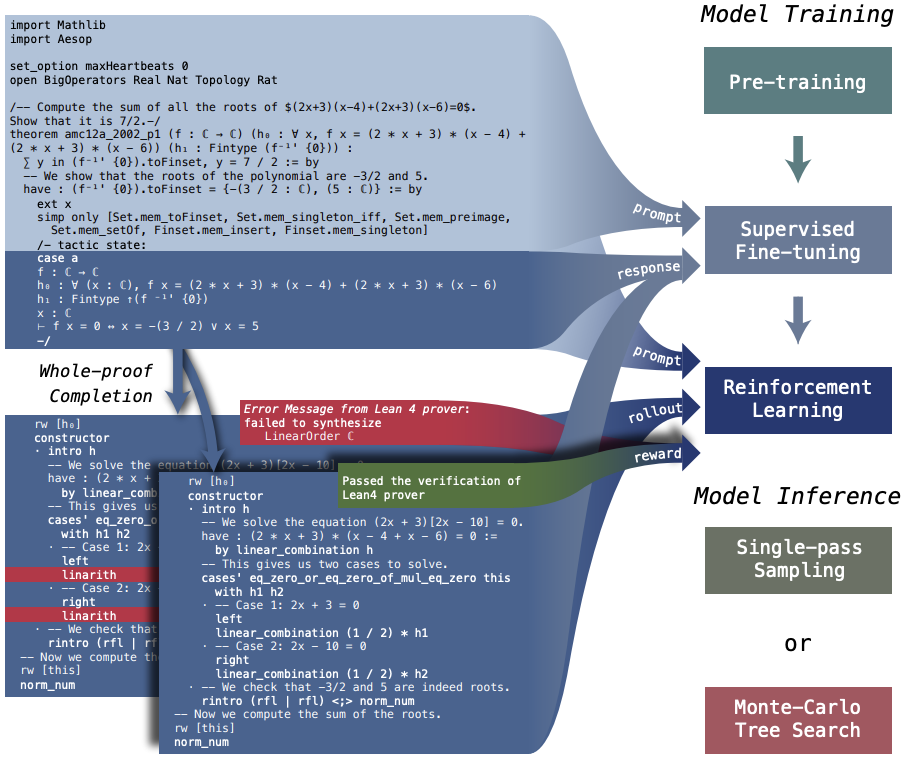
\includegraphics[height = 4in]{\images/DeepSeek2}}

\vfill
DeepSeek does not use tree-search bootstrapping.

\slide{GRPO RL Optimization}

DeepSeek uses a variant of PPO called GRPO for RL.

\vfill
PPO is an advantage-actor-critic policy gradient algorithm.

$$\nabla_\Theta R(\pi_\Theta) = E_{s_t,a_t}\left[(\ln \pi_\Theta(a_t)) \hat{A}(s_t,a_t)\right]$$

\vfill
For a fixed advantage $\hat{A}(s_t,a_t)$ this gradient is a nonlinear function of $\Theta$.

\vfill
Rather than take a single linear step, PPO moves some distance along this nonlinear path.

\vfill
In AlphaZero this happens when elements of the replay buffer are reused.

\slide{LLM Proofs Without Formal Verification}

The blog post on alphaproof also says that they are experimenting with proofs generated entirely by natural language --- no formal verification.  They say:

\vfill

\begin{quotation}
We also tested [the language only] approach on this year’s IMO problems and the results showed great promise.
\end{quotation}

\slide{OpenAI o1 as a Proof Assistant}

Terence Tao has a Mastodon post evauating o1 as an assistant for research mathematicians. He says:

\vfill
\begin{quotation}
The experience seemed roughly on par with trying to advise a mediocre, but not completely incompetent, (static simulation of a) graduate student.
\end{quotation}

\slide{Formal Language vs. Natural Language}

In chess, Go, shogi, it is trivial to define the moves of the game in a formal language.

\vfill
This is also true in the game of Diplomacy where orders to generals have a fixed grammar and even statements
in negotiation are best viewed as proposals for orders.

\vfill
Mathematics can also be defined in terms of formal language.

\vfill
This would suggest that English/formal translation is ultimately not difficult and the
hard challenge is solving the game defined in the rules of the formal language.

\slide{Formal Language vs. Natural Language}

An argument in favor of LLM reasoning (rather than formal reasoning) is that mathematics requires intuition and intuition is not formal.

\vfill
Time will tell if intuition is best captured in natural language or in some internal language with formal grammar but imprecise semantics.

\slide{Algorithms in the Age of LLMs}

What is the role of algorithms in the age of LLMs?

\vfill
It seems unlikely that LLMs will ever replace compilers which, by deep model standards, are {\bf incredibly efficient}.

\vfill
Lean includes certain decision procedures such as one for deciding whether an linear equation
follows from a given set of linear equations and inequalities.

\vfill
AlphaGeometry (a DeepMind geometry theorem prover) relies on Wu's algorithm from the 1970s.

\slide{Can Lean be Strengthened?}

There are well-known algorithms for general logic that are used to great effect in SMT (Sat Modulo a Theory) software verifiers
(such as Microsoft's Z3).

\vfill
Alfred is a system that I have built based on general logic algorithms not present in Lean.

\vfill
Alfred is intended as a competitor for Lean.

\slide{The Schroder-Berstein Theorem}

For any two sets $s$ and $w$, if there exists an injection of $s$ into $w$ and an injection of $w$ into $s$ then there exists a bijection between $s$ and $w$.

\slide{The Schroder-Berstein Theorem}

\centerline{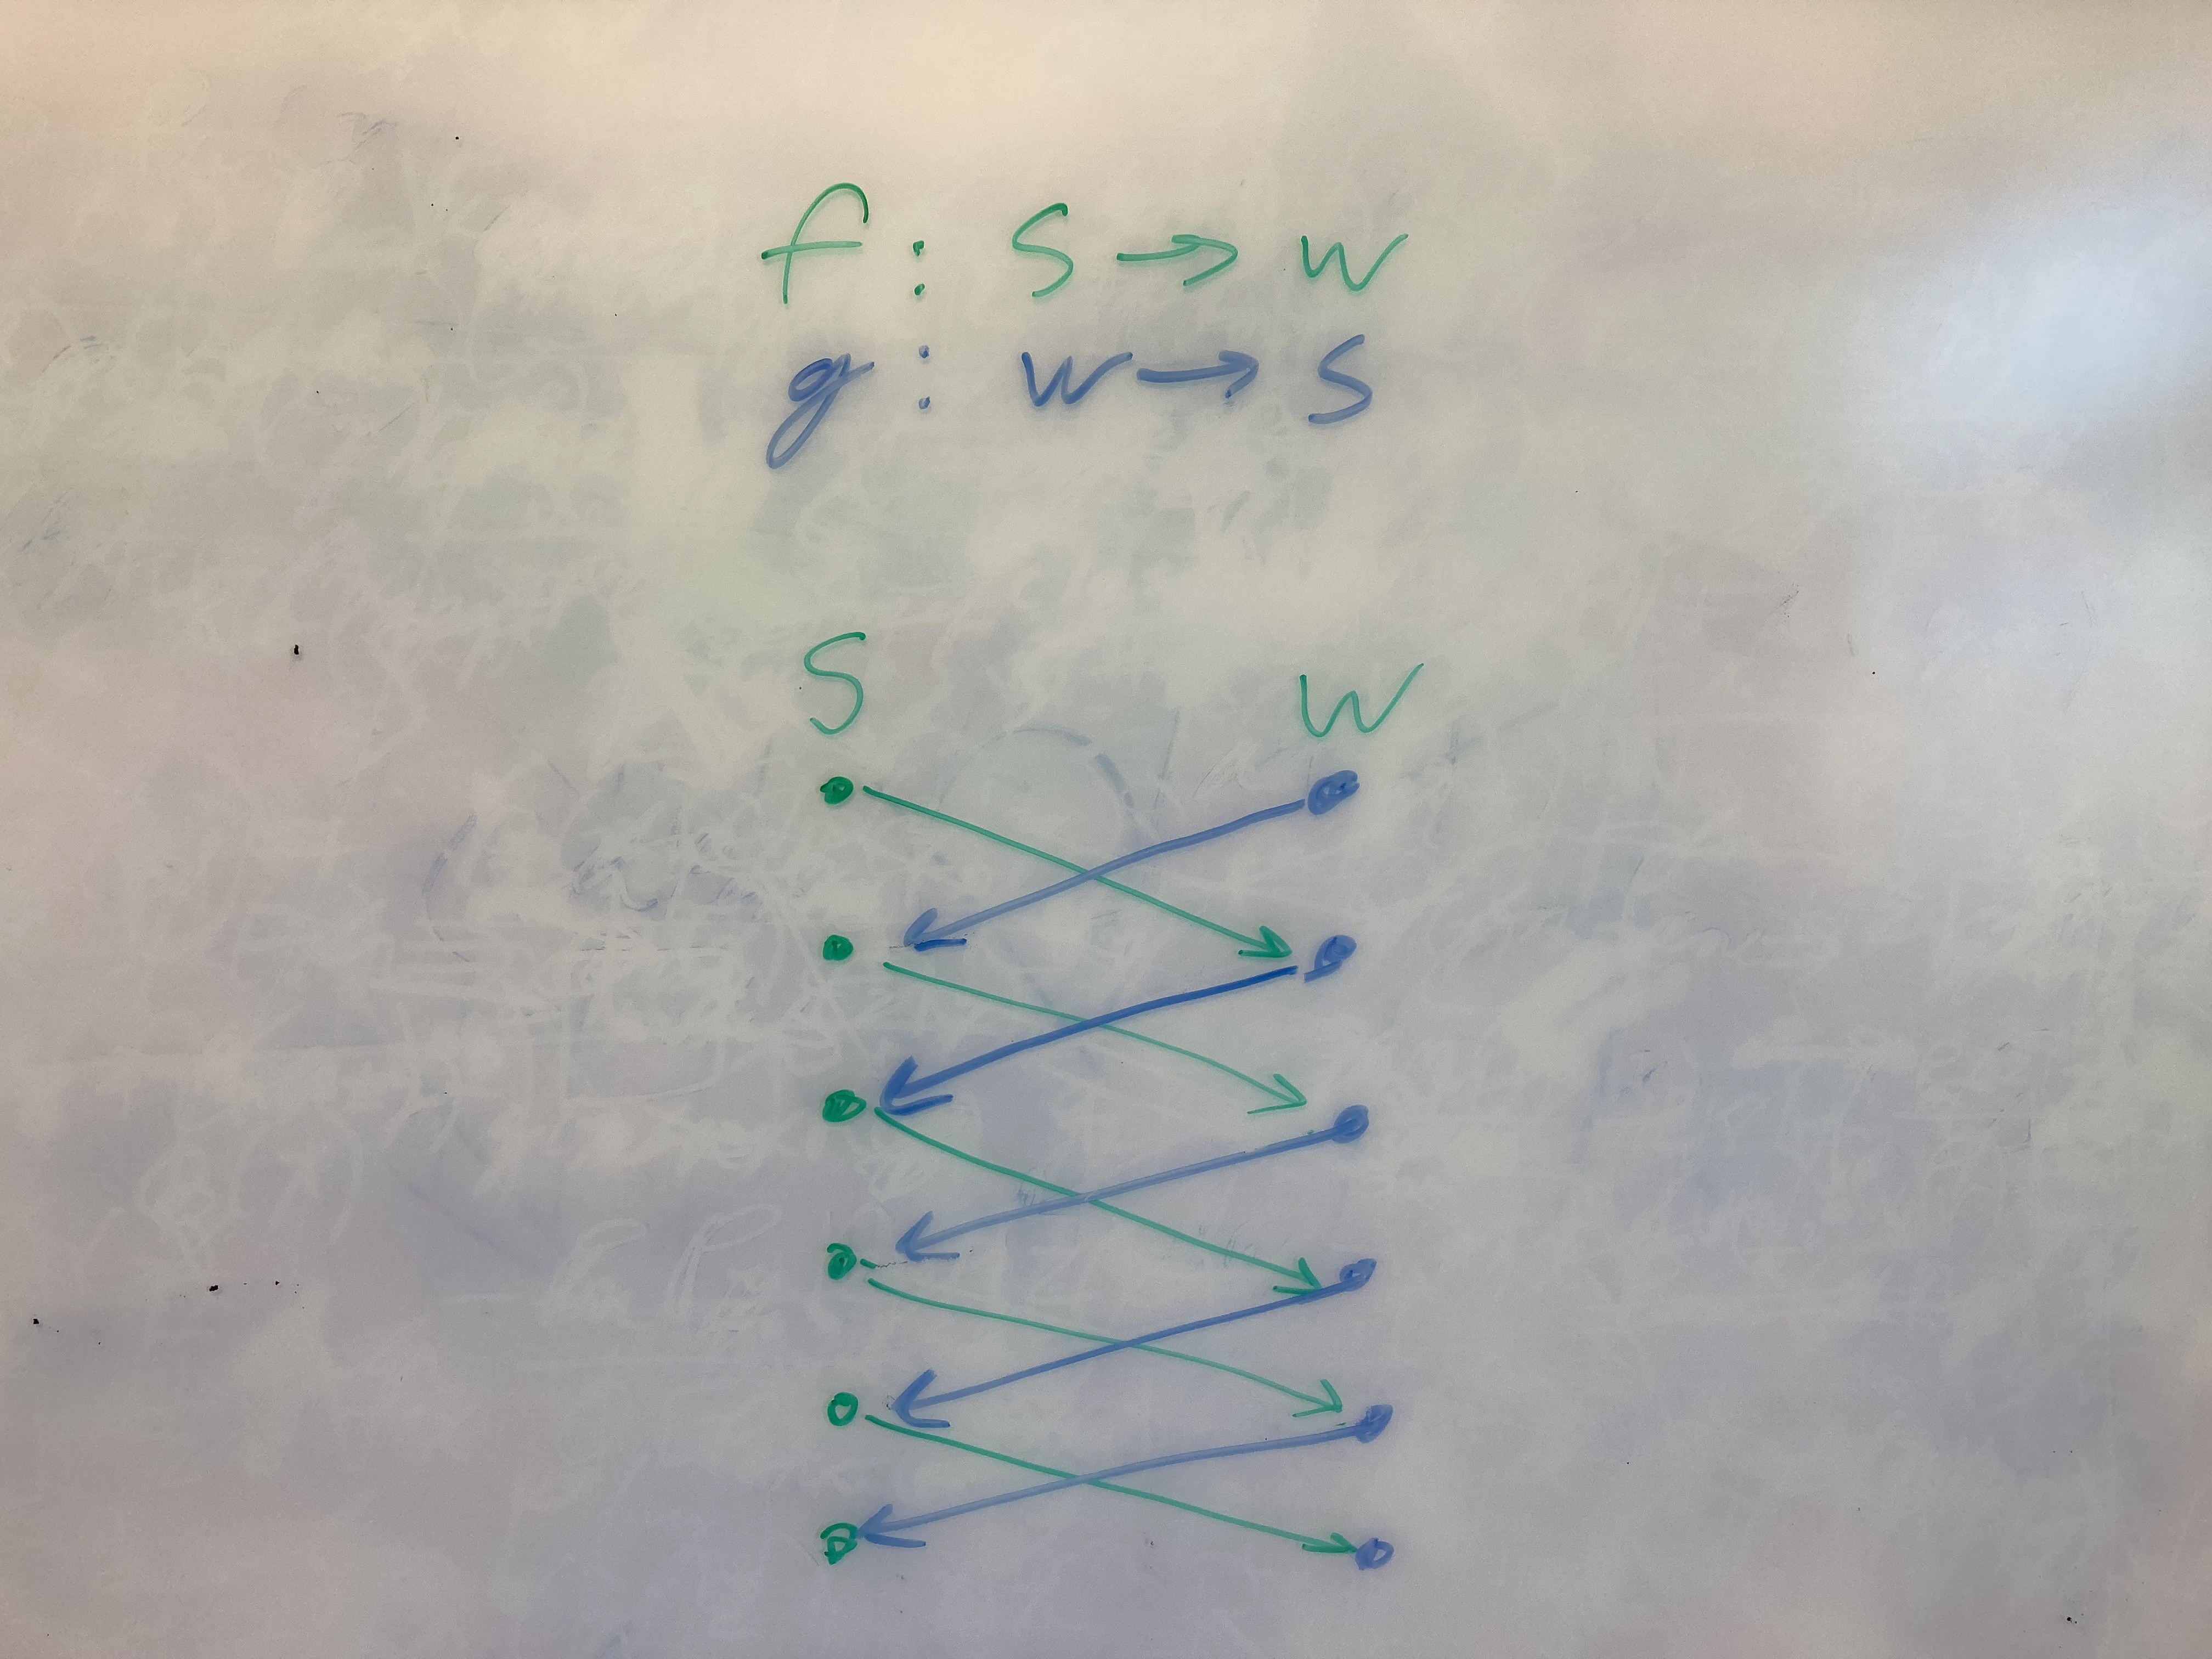
\includegraphics[width = 6.5in]{\images/SB4}}

\slide{The Schroder-Berstein Theorem}

\centerline{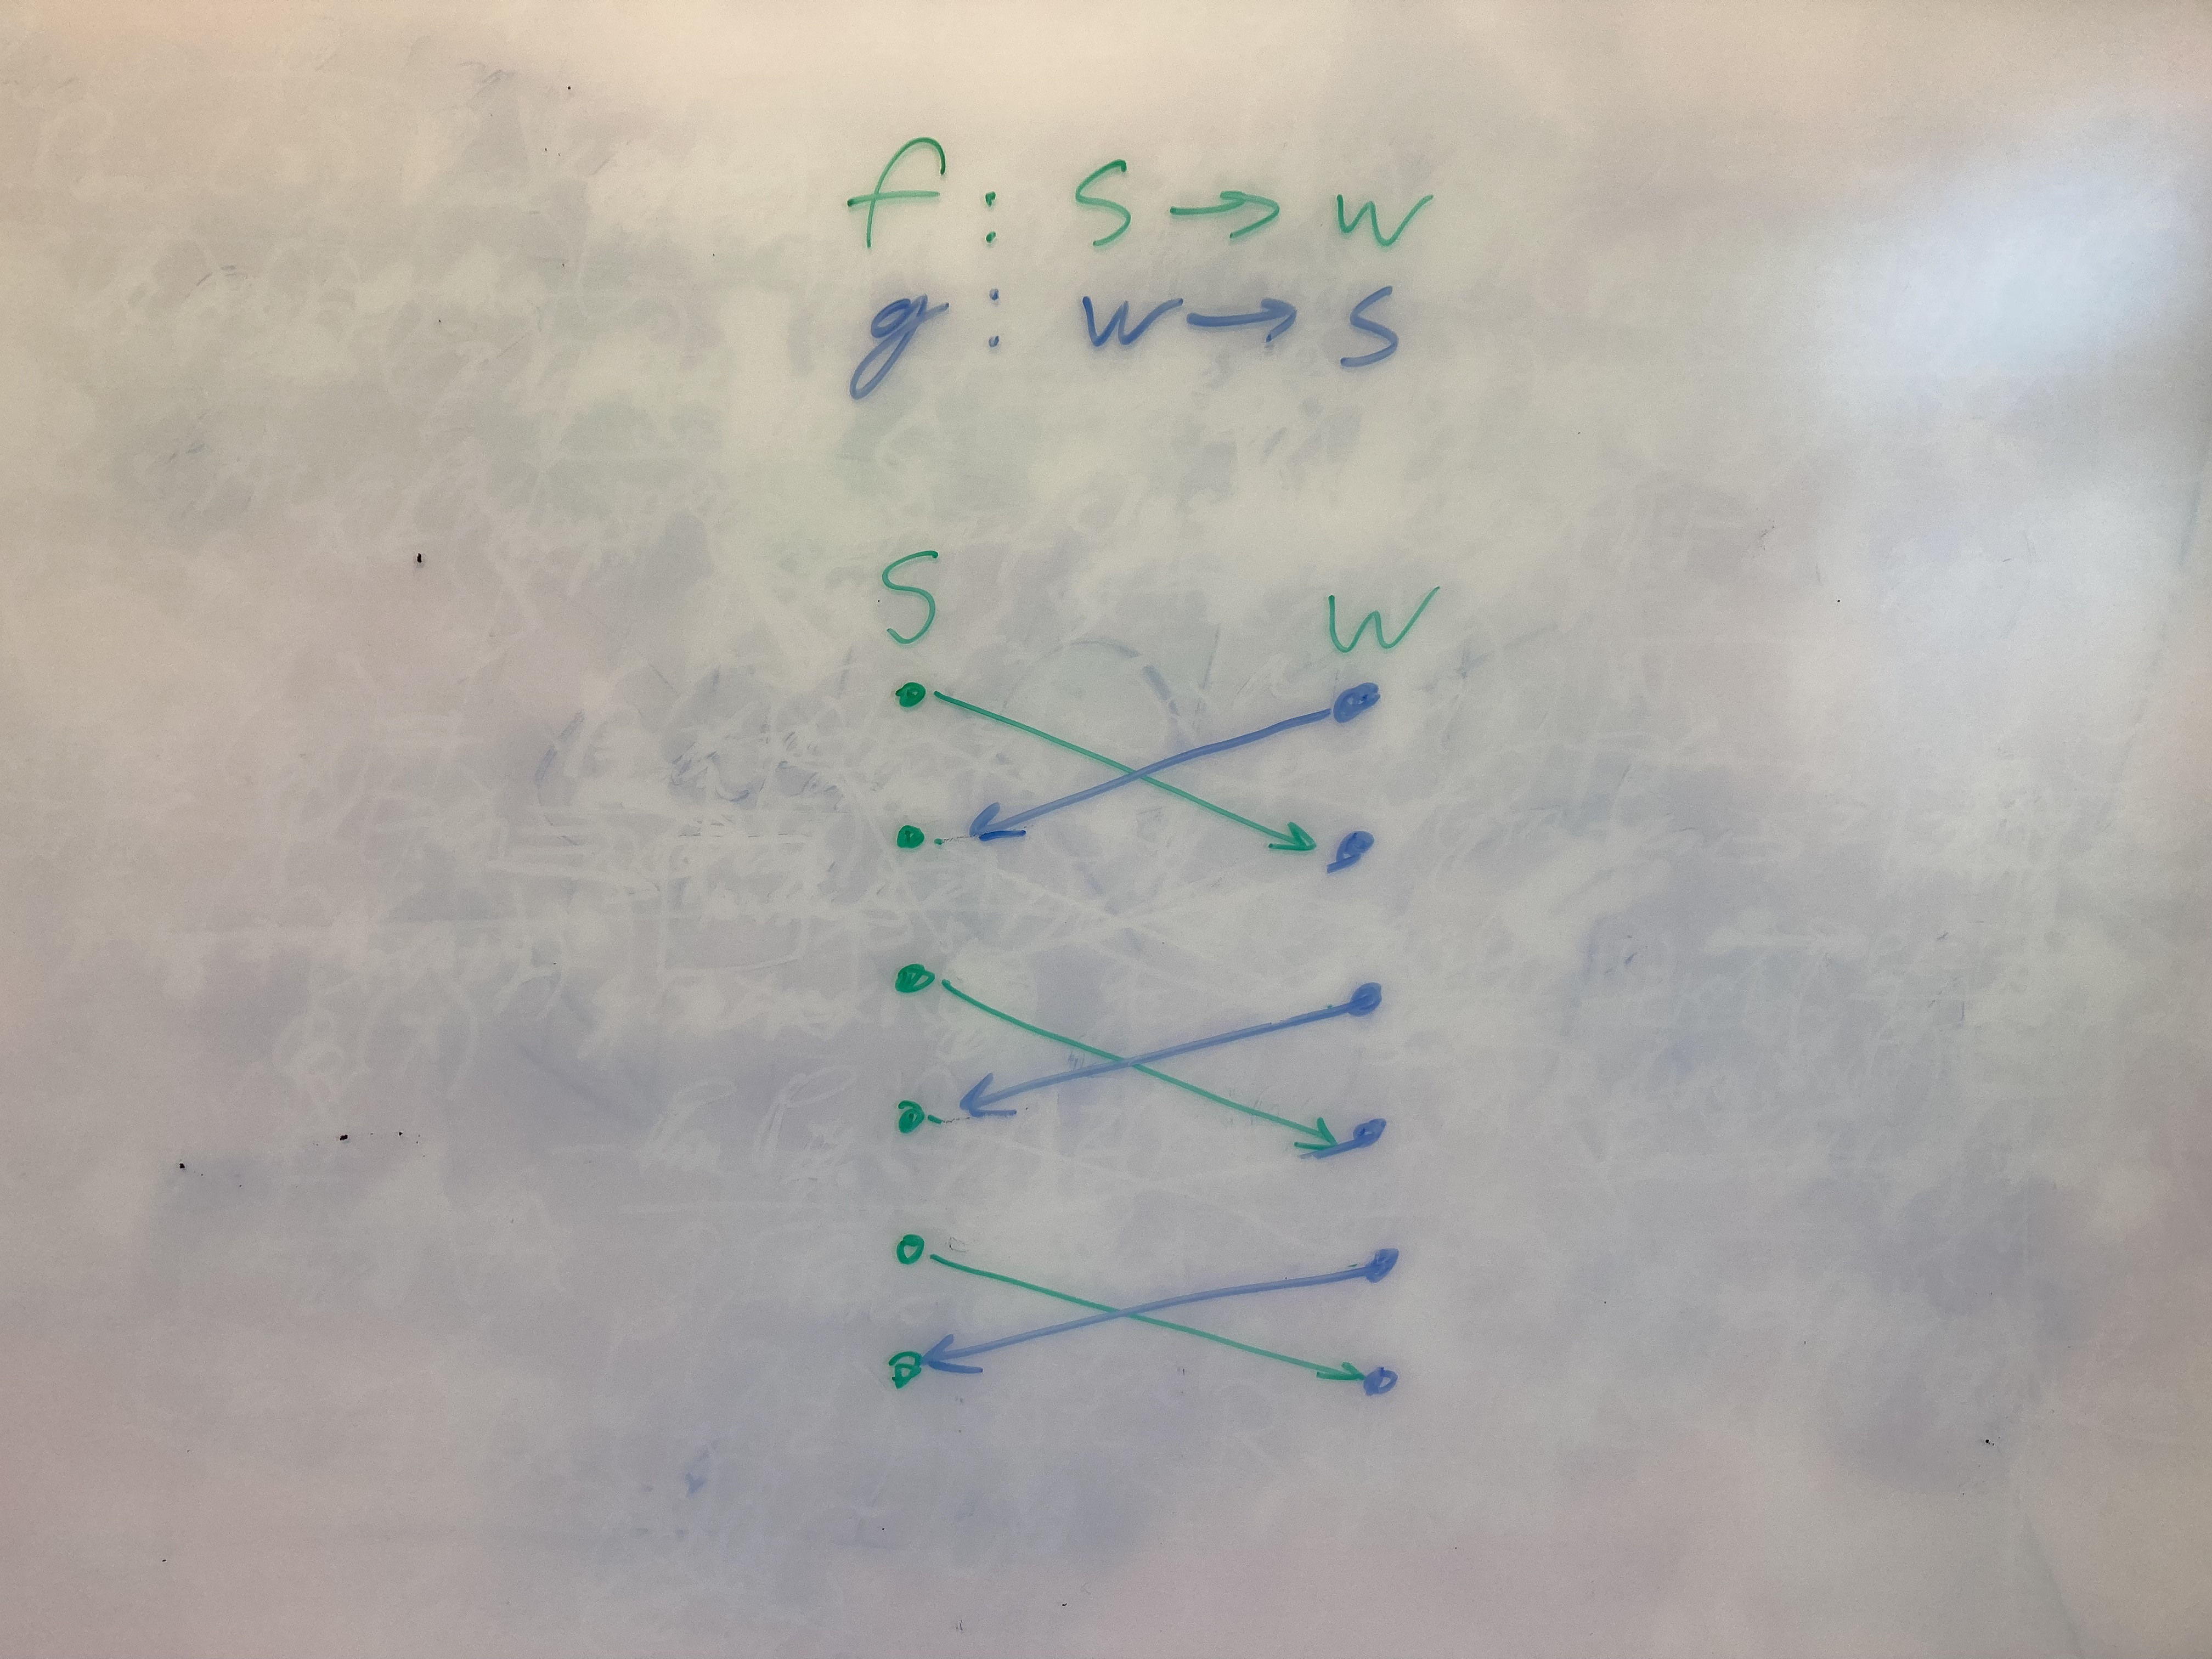
\includegraphics[width = 6.5in]{\images/SB3}}


\slide{The Schroder-Berstein Theorem in Alfred}

\centerline{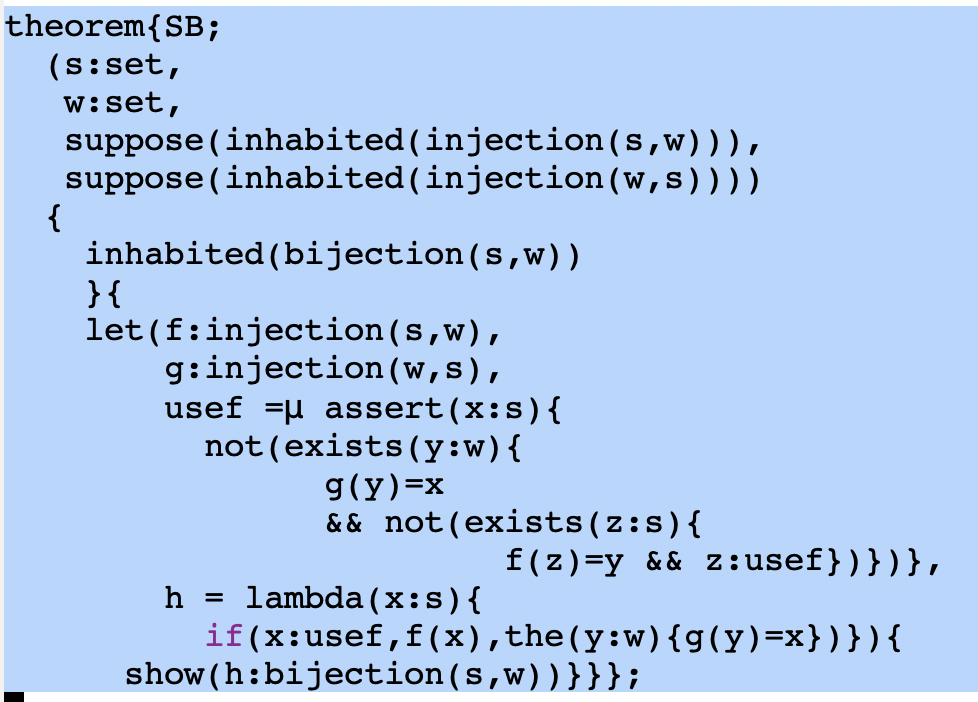
\includegraphics[width = 6.5in]{\images/AlfSchroeder}}

\slide{The Schroeder-Bernstein Theorem from Lean's MathLib}

\centerline{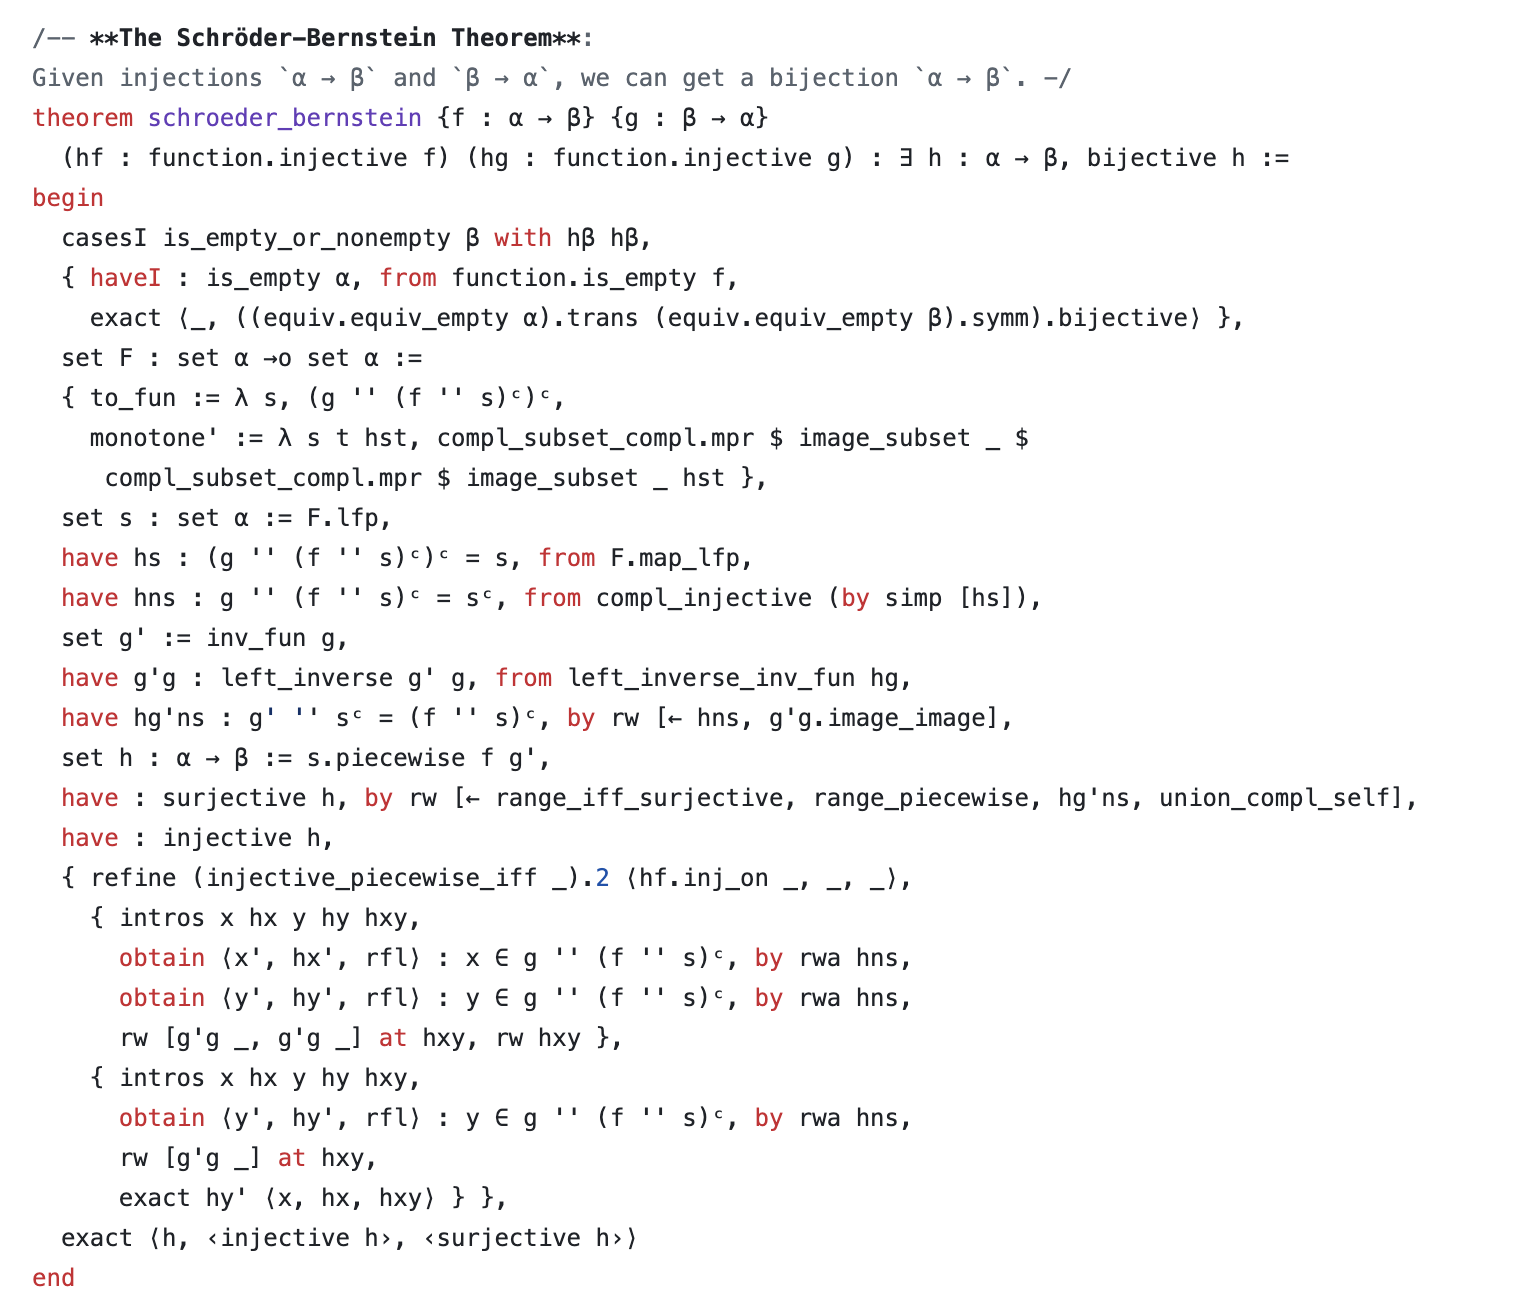
\includegraphics[width = 6.2in]{\images/Schroeder}}

\slide{END}

}
\end{document}



